%% BioMed_Central_Tex_Template_v1.06
%%                                      %
%  bmc_article.tex            ver: 1.06 %
%                                       %

%%IMPORTANT: do not delete the first line of this template
%%It must be present to enable the BMC Submission system to
%%recognise this template!!

%%%%%%%%%%%%%%%%%%%%%%%%%%%%%%%%%%%%%%%%%
%%                                     %%
%%  LaTeX template for BioMed Central  %%
%%     journal article submissions     %%
%%                                     %%
%%          <8 June 2012>              %%
%%                                     %%
%%                                     %%
%%%%%%%%%%%%%%%%%%%%%%%%%%%%%%%%%%%%%%%%%

%%%%%%%%%%%%%%%%%%%%%%%%%%%%%%%%%%%%%%%%%%%%%%%%%%%%%%%%%%%%%%%%%%%%%
%%                                                                 %%
%% For instructions on how to fill out this Tex template           %%
%% document please refer to Readme.html and the instructions for   %%
%% authors page on the biomed central website                      %%
%% https://www.biomedcentral.com/getpublished                      %%
%%                                                                 %%
%% Please do not use \input{...} to include other tex files.       %%
%% Submit your LaTeX manuscript as one .tex document.              %%
%%                                                                 %%
%% All additional figures and files should be attached             %%
%% separately and not embedded in the \TeX\ document itself.       %%
%%                                                                 %%
%% BioMed Central currently use the MikTex distribution of         %%
%% TeX for Windows) of TeX and LaTeX.  This is available from      %%
%% https://miktex.org/                                             %%
%%                                                                 %%
%%%%%%%%%%%%%%%%%%%%%%%%%%%%%%%%%%%%%%%%%%%%%%%%%%%%%%%%%%%%%%%%%%%%%

%%% additional documentclass options:
%  [doublespacing]
%  [linenumbers]   - put the line numbers on margins

%%% loading packages, author definitions

%\documentclass[twocolumn]{bmcart}% uncomment this for twocolumn layout and comment line below
\documentclass{bmcart}

%%% Load packages
\usepackage{amsthm,amsmath}
\usepackage{hyperref}
%\RequirePackage[numbers]{natbib}
%\RequirePackage[authoryear]{natbib}% uncomment this for author-year bibliography
%\RequirePackage{hyperref}
\usepackage[utf8]{inputenc} %unicode support
%\usepackage[applemac]{inputenc} %applemac support if unicode package fails
%\usepackage[latin1]{inputenc} %UNIX support if unicode package fails

%for abbreviations item list
\usepackage{blindtext}
\usepackage{enumitem}
\usepackage{xcolor}
\usepackage{graphicx}
%for url
\usepackage{hyperref}
%
%include figure 
%\usepackage{graphicx}

%%%%%%%%%%%%%%%%%%%%%%%%%%%%%%%%%%%%%%%%%%%%%%%%%
%%                                             %%
%%  If you wish to display your graphics for   %%
%%  your own use using includegraphic or       %%
%%  includegraphics, then comment out the      %%
%%  following two lines of code.               %%
%%  NB: These line *must* be included when     %%
%%  submitting to BMC.                         %%
%%  All figure files must be submitted as      %%
%%  separate graphics through the BMC          %%
%%  submission process, not included in the    %%
%%  submitted article.                         %%
%%                                             %%
%%%%%%%%%%%%%%%%%%%%%%%%%%%%%%%%%%%%%%%%%%%%%%%%%


%\def\includegraphic{}
%\def\includegraphics{}

%%% Put your definitions there:
\startlocaldefs
\endlocaldefs

\usepackage{xcolor}
\newcommand{\comment}[1]{ \color{red} #1 \color{black}}
\newcommand{\reply}[1]{ \color{blue} [#1] \color{black}}
\newcommand{\revision}[1]{ \color{blue} [#1] \color{black}}
\newcommand{\eqn}[1]{Eq.~(\ref{#1})}
\newcommand{\fig}[1]{Fig.~\ref{#1}}
\newcommand{\tab}[1]{Table~\ref{#1}}
\newcommand{\sect}[1]{Section~\ref{#1}}

%%% Begin ...
\begin{document}

%%% Start of article front matter
\begin{frontmatter}

\begin{fmbox}

\dochead{Research}

%%%%%%%%%%%%%%%%%%%%%%%%%%%%%%%%%%%%%%%%%%%%%%
%%                                          %%
%% Enter the title of your article here     %%
%%                                          %%
%%%%%%%%%%%%%%%%%%%%%%%%%%%%%%%%%%%%%%%%%%%%%%

\title{An Oscillating Reaction Network With an Exact Closed Form Solution in the Time Domain Solution}

%%%%%%%%%%%%%%%%%%%%%%%%%%%%%%%%%%%%%%%%%%%%%%
%%                                          %%
%% Enter the authors here                   %%
%%                                          %%
%% Specify information, if available,       %%
%% in the form:                             %%
%%   <key>={<id1>,<id2>}                    %%
%%   <key>=                                 %%
%% Comment or delete the keys which are     %%
%% not used. Repeat \author command as much %%
%% as required.                             %%
%%                                          %%
%%%%%%%%%%%%%%%%%%%%%%%%%%%%%%%%%%%%%%%%%%%%%%

\author[
  addressref={aff1},                   % id's of address
  corref={aff1},
  email={jlheller@uw.edu}
  %{aff1,aff2}
% corref={aff1},                       % id of corresponding %address, if any
% noteref={n1},                        % id's of article notes, %if any
%  email={jane.e.doe@cambridge.co.uk}   % email address
]{\inits{J.L.H.}\fnm{Joseph} \snm{Hellerstein}}
%\author[
%  addressref={aff1},                   % id's of address
%]{\inits{H.M.S.}\fnm{Herbert M.} \snm{Sauro}}
%\author[
%  addressref={aff2},
  %corref={aff2},
  %email={joseph.hellerstein@gmail.com}
%]{\inits{J.H.}\fnm{Joseph L.} \snm{Hellerstein}}

%%%%%%%%%%%%%%%%%%%%%%%%%%%%%%%%%%%%%%%%%%%%%%
%%                                          %%
%% Enter the authors' addresses here        %%
%%                                          %%
%% Repeat \address commands as much as      %%
%% required.                                %%
%%                                          %%
%%%%%%%%%%%%%%%%%%%%%%%%%%%%%%%%%%%%%%%%%%%%%%

\address[id=aff1]{%                           % unique id
  \orgdiv{eScience Institute},             % department, if any
  \orgname{University of Washington},          % university, etc
  \city{Seattle},                              % city
  \cny{USA}                                    % country
}
%\address[id=aff2]{%
%  \orgdiv{eScience Institute},
%  \orgname{University of Washington},
%  %\street{},
%  %\postcode{}
%  \city{Seattle},
%  \cny{USA}
%}

%%%%%%%%%%%%%%%%%%%%%%%%%%%%%%%%%%%%%%%%%%%%%%
%%                                          %%
%% Enter short notes here                   %%
%%                                          %%
%% Short notes will be after addresses      %%
%% on first page.                           %%
%%                                          %%
%%%%%%%%%%%%%%%%%%%%%%%%%%%%%%%%%%%%%%%%%%%%%%

%\begin{artnotes}
%%\note{Sample of title note}     % note to the article
%\note[id=n1]{Equal contributor} % note, connected to author
%\end{artnotes}

\end{fmbox}% comment this for two column layout

%%%%%%%%%%%%%%%%%%%%%%%%%%%%%%%%%%%%%%%%%%%%%%%
%%                                           %%
%% The Abstract begins here                  %%
%%                                           %%
%% Please refer to the Instructions for      %%
%% authors on https://www.biomedcentral.com/ %%
%% and include the section headings          %%
%% accordingly for your article type.        %%
%%                                           %%
%%%%%%%%%%%%%%%%%%%%%%%%%%%%%%%%%%%%%%%%%%%%%%%

\begin{abstractbox}
\begin{abstract} % abstract
\parttitle{Background} Oscillatory behavior is critical to many life sustaining processes such as cell cycles, circadian rhythms, and notch signaling. Important biological functions depend on the characteristics of these oscillations (hereafter, oscillation characteristics or OCs): frequency (e.g., event timings), amplitude (e.g., signal strength), and phase (e.g., event sequencing).
\parttitle{Results} 
We conduct a theoretical study of an oscillating reaction network to quantify the relationships between oscillation characteristics and the structure and parameters of the reaction network. We develop a two species ($S_1, S_2$) reaction network whose dynamics can be described by a system of linear differential equations. We solve this system to obtain exact, closed-form formulas for our network's OCs. These formulas are used to develop the {\tt designOscillator} algorithm that designs oscillators by finding values of parameters of our reaction network that achieve desired OCs. 
\parttitle{Conclusions} The OC formulas are employed to analyze the roles of the reactions in the network, and to comment on other studies of oscillatory reaction networks. For example, others have stated that nonlinear dynamics are required to create oscillations in reaction networks. We refute this, at least in theory, since our oscillatory reaction network has linear dynamics. Our formulas also show that the rate of negative feedback must exceed the rate of positive feedback in our reaction network.



\end{abstract}

%%%%%%%%%%%%%%%%%%%%%%%%%%%%%%%%%%%%%%%%%%%%%%
%%                                          %%
%% The keywords begin here                  %%
%%                                          %%
%% Put each keyword in separate \kwd{}.     %%
%%                                          %%
%%%%%%%%%%%%%%%%%%%%%%%%%%%%%%%%%%%%%%%%%%%%%%

\begin{keyword}
\kwd{Systems biology}
\end{keyword}

% MSC classifications codes, if any
%\begin{keyword}[class=AMS]
%\kwd[Primary ]{}
%\kwd{}
%\kwd[; secondary ]{}
%\end{keyword}

\end{abstractbox}
%
%\end{fmbox}% uncomment this for two column layout

\end{frontmatter}

%%%%%%%%%%%%%%%%%%%%%%%%%%%%%%%%%%%%%%%%%%%%%%%%
%%                                            %%
%% The Main Body begins here                  %%
%%                                            %%
%% Please refer to the instructions for       %%
%% authors on:                                %%
%% https://www.biomedcentral.com/getpublished %%
%% and include the section headings           %%
%% accordingly for your article type.         %%
%%                                            %%
%% See the Results and Discussion section     %%
%% for details on how to create sub-sections  %%
%%                                            %%
%% use \cite{...} to cite references          %%
%%  \cite{koon} and                           %%
%%  \cite{oreg,khar,zvai,xjon,schn,pond}      %%
%%                                            %%
%%%%%%%%%%%%%%%%%%%%%%%%%%%%%%%%%%%%%%%%%%%%%%%%

%%%%%%%%%%%%%%%%%%%%%%%%% start of article main body
% <put your article body there>


%%%%%%%%%%%%%%%%
%% Background %%
%%

\section*{Background}
Oscillatory behavior is critical to many life sustaining processes. Examples include: cell cycles \cite{Murray1991}, circadian rhythms \cite{capper_overview_2001}, notch signaling in the development of the nervous system \cite{wang_neural_2011}, tissue development \cite{goodwin1969}, and gene transcription \cite{nelson2004}.
%Biological oscillators are also important elements of modules in synthetic biology \cite{benner_synthetic_2005}.
Biological oscillators are also important elements in building applications in synthetic biology \cite{Perry2012, zhang_independent_2022, Elowitz2000}.

The characteristics of biological oscillations often have critical biological functions. Frequency is used to control the times at which events are initiated, such as circadian cycles and chromatin modifications \cite{venkatachalam2022}. Amplitude controls the strength of signaling \cite{mahrou_degradation-driven_2022}. Phase plays a role in the sequencing of processes within the cell cycle \cite{Ball2011}. Since biological oscillators typically cause changes in the concentration of chemical species, these oscillators must have a DC offset so that values are non-negative. Collectively, we refer to frequency, amplitude, phase, and DC offset as {\bf oscillation characteristics (OCs)}.

%The foregoing highlights the value of being able to make quantitative predictions of OCs from the structure and parameterization (e.g., values of kinetic constants) of a reaction network. There is substantial literature on oscillations in biological systems. This literature can be organized into several themes: (a) qualitative characterizations of oscillating networks; (b) building biological oscillators; and (c) modeling biological oscillators.

One way to understand the relationship between an oscillating reaction network and its OCs is to construct a closed-form, time-domain solution of the network's behavior in terms of parameters such as kinetic constants and initial concentrations of chemical species. From these mathematical expressions, we obtain insights such as: (a) if one or more reactions are unnecessary to achieve oscillations; (b) relationships between the kinetic constants of reactions; and (c) how to assign values to network parameters so as to achieve desired OCs.

Many researchers have investigated structural aspects of oscillating reaction networks. These structures include: positive feedback, negative feedback, balancing reaction rates, and ultrasensitivity
\cite{cao2016, Li2018, lenz_temporal_2011, HoonHa2012, tatka_cesium_2023}. Others have built biological oscillators \cite{atkinson_development_2003, Ball2011,  Elowitz2000, nakajima2005, Perry2012, rosier_how_2015,  weitz2014}. But neither kind of investigation addresses our interest in a closed-form, time-domain solution that relates parameters of a reaction network to its OCs.

More relevant to our work are quantitative models of biological oscillators. For the most part, existing models are systems of nonlinear ordinary differential equations \cite{huxley1952, Goodwin1965, heinrich1977, Goldbeter1991, rumbell_dimensions_2019, sadeghpour_bistability_2017}. The complexity of these models prohibits the construction of a closed-form, time-domain solution.

We are aware of two approaches that circumvent the limitations of nonlinear ODEs. The first uses an empirical approach, system identification, to construct a linear model that approximates the nonlinear system  (e.g., \cite{mahrou2022}). Models constructed in this way provide accurate predictions near the operating point at which system identification is done. The second approach constructs a linear approximation to a nonlinear ODE (e.g.,  \cite{kut_analytical_2009}). Typical approximations make assumptions about relative reaction rates and/or magnitudes of species concentrations. In both cases, the construction of a linear models greatly reduces the complexity of the mathematical expressions, and this in turn makes it possible to obtain a closed-form, time-domain solution. However, the approximations limit the extent to which the resulting mathematical expressions provide useful interpretations of how the parameters of the reaction network affect OCs.

The present work is a theoretical study in that we do not build a biological oscillator. Rather, we develop an oscillating reaction network whose dynamics are described by a system of linear ordinary differential equations (ODEs). The network is consistent with biological networks (hereafter, {\bf biologically feasible}) in that: (a) species concentrations are not negative; and (b) reactions have rate laws that are used in models of biological systems (e.g., BioModels \cite{malik-sheriff_biomodels-15_2020}). We solve the ODEs to obtain an {\em exact} closed-form, time-domain solution, and then construct formulas that relate OCs to the parameters of our reaction network. These formulas provide considerable insight into how parameters of the reaction network affect OCs, something that likely cannot be determined from the network structure alone. Further, we use the formulas to develop an algorithm for designing oscillators that achieve desired oscillation characteristics.

    %There are two parts to creating a RNCO. The first is to create a reaction network with {\em predictable} oscillations. That is, we can predict the amplitude, frequency, and phase of oscillations from the network structure and parameter values. The second part is estimating the parameters of the reaction network that will produce a desired oscillation--amplitude, frequency, and phase.\begin{itemize} \item Propose an oscillating reaction network in which can specify the design parameters to achieve a desired amplitude, frequency, and phase of oscillations. Must be a biologically feasible network in the sense that: (a) species concentrations are non-negative and (b) reaction rate laws are consistent with those of existing models of biological networks. \item The actual construction of a gene network (or other biological network) is beyond the scope of this paper. \item Instead we propose a simple oscillating reaction network in we can control the amplitude, frequency, and phase of oscillations. \item To achieve simultaneous control over amplitude, phase, and frequency, we construct a network whose dynamics can be represented by a linear ODE. \end{itemize}

%\cite{zhang_independent_2022} summarizes well current research on biological oscillating networks, that proposed “synthetic oscillations are difficult to control”. Analogously, for natural biological oscillators, we have mostly a qualitatively understanding of how network structure and parameters affect oscillator characteristics.a


%%%%%%%%%%%%%%%%%%%%%%%%%%%%%%%%%%%%%%%%%%%%%%%
\section*{Methods}
Our method is to propose a reaction network whose kinetics are linear and biologically feasible. We solve this system of linear ODEs (an initial value problem) to obtain formulas that relate OCs to parameters of the reaction network. Finally, we develop an algorithm for designing an oscillator with desired OCs by properly assigning values to parameters of the reaction network.

\subsection*{Reaction Network}
This section develops a biologically feasible reaction network whose kinetics can be described as a system of linear ODEs. A system of linear ODEs can be expressed in matrix form as: 
\begin{equation}
\dot{{\bf x}}(t) = {\bf A} {\bf x}(t) + {\bf u},
\label{eq:linear}
\end{equation}
where ${\bf x} (t) = \{x_n (t)\}$ is an $N$ 
dimension vector of time varying of 
species concentrations; $\dot {\bf x} (t)$
is the time derivative of ${\bf x}(t)$; ${\bf A} = \{a_{ij} \}$ is an $N \times N$ Jacobian matrix of constants;
and ${\bf u}$ is an $N$ dimensional vector of constants that are forced inputs. We want to construct a reaction network that has a sustained oscillation. Since this is a linear system, the oscillations will be sinusoids.

From the foregoing, we have the following constraints:
\begin{itemize}
    \item {\bf C1}: Rate laws in the reaction network are a linear function of the concentrations of $x_n$(t).
    \item {\bf C2}: $x_n(t) \geq 0$ so that the reaction network is biologically feasible.
\end{itemize}

We simplify the problem by having $N=2$, since this is sufficient to obtain oscillations. This means that the eigenvalues of ${\bf A}$ 
must be pure imaginary numbers. Let $\tau = a_{11} + a_{22}$ be the trace of ${\bf A}$, and 
$\Delta = a_{11} a_{22} - a_{12} a_{21}$ be the
determinant of ${\bf A}$. 
The eigenvalues are complex conjugates $\lambda_1, \lambda_2$ such that
\begin{equation*}
\lambda_n  = \frac{\tau}{2}  \pm \frac{\sqrt{\tau^2 - 4 \Delta}}{2}
\end{equation*}
Clearly, we obtain pure imaginary eigenvalues only if $\tau =  0$ and $\Delta > 0$. Thus, we add the constraints
\begin{itemize}
    \item {\bf C3}: $\tau = 0$, where $\tau$ is the trace of ${\bf A}$.
       \item {\bf C4}: $\Delta > 0$, where $\Delta$ is the determinant of ${\bf A}$.
\end{itemize}
With these constraints, $\lambda_n = \pm \theta i,$ where $\theta = \sqrt{\Delta}.$

We use $k_i \geq 0$ to specify kinetics constants, where $i$ indexes the reaction in the network. Let $S_n$ be a chemical species whose time varying concentration is the state variable $x_n(t)$ for $n=\{1,2\}.$ We start by having two-way interactions between the species. Rate laws are specified above the reaction arrow.
\begin{itemize}
    \item $R_1: S_1 \xrightarrow{k_1 S_1} S_2$
    \item $R_2: S_2 \xrightarrow{k_2 S_2} S_1$
\end{itemize}
The foregoing reactions have mass action kinetics, which is widely used in models of chemical systems.
With just these reactions, ${\bf A}$ is
$$\left( \begin{matrix}
     - k_1 & k_2  \\
     k_1 & -k_2 
\end{matrix} \right)$$
Clearly, C3 does not hold: $\tau < 0$ since both terms in the diagonal are negative. To address this, we make $a_{11}$ positive by adding an autocatalysis reaction, a kind of reaction that
arises in many biological oscillators \cite{novichkov_autocatalytic_2021}.
\begin{itemize}
    \item $R_3: S_1 \xrightarrow{k_3 S_1} 2 S_1$
\end{itemize}
and so ${\bf A}$ becomes
$$\left( \begin{matrix}
     k_3 - k_1 & k_2  \\
     k_1 & -k_2
\end{matrix} \right)$$
which is positive with appropriate choices of the $k_i$.

Since $R_3$ synthesizes $S_1$, we need a reaction that degrades $S_1$ in order for the system to be stable. If we use mass action kinetics for this reaction, $kS_1$, it changes $a_{11}$ to $k_1-k_2-k$, which makes it more difficult to satisfy C3. An alternative is a fixed degradation rate of $k_4 > 0$, where $k_4 = u_1$ is the first element of the vector ${\bf u}$ in \eqn{eq:linear}.
\begin{itemize}
    \item $R_4$: $S_1\xrightarrow{k_4}\emptyset$
\end{itemize}
Examples of fixed rate degradation reactions in BioModels are: reaction {\tt reaction\_0} in {\tt BIOMD0000000112}, reaction
{\tt ATP\_Jerp} in {\tt BIOMD0000000059},
and reaction
\linebreak
{\tt inhibition\_parameter2} in {\tt BIOMD0000000224}.

We must still address constraint C4, that the determinant is positive. This requires that $a_{12} a_{21} < 0,$ which mean that one of $a_{12}, a_{21}$ is positive and the other is negative. We make $a_{21} < 0$ by degrading $S_2$ at a rate controlled by $S_1$.
That is,
\begin{itemize}
    \item $R_5$: $S_2 \xrightarrow{k_5 S_1}\emptyset$
\end{itemize}
Having the degradation of one chemical species controlled by another chemical species is common in BioModels. Some examples are: the {\tt fast} reaction in model {\tt BIOMD0000000108}, reaction {\tt r10} in {\tt BIOMD0000000145},
and reaction {\tt RuBisCO\_5\_EOP} in {\tt BIOMD0000000392}. With the addition of reaction $R_5$,
${\bf A}$ becomes
$$\left( \begin{matrix}
     k_3 - k_1 & k_2  \\
     k_1 - k_5 & -k_2
\end{matrix} \right).$$

The final reaction in our network compensates for degrading $S_2$ by synthesizing this species at a fixed rate. That is,
\begin{itemize}
    \item $R_6$: $\emptyset \xrightarrow{k_6} S_2$
\end{itemize}
(We do not explicitly cite examples of similar synthesis reactions since they are widely used in BioModels.)
From this, we observe that 
\begin{equation}
   {\bf u} = \left( \begin{matrix}
       -k_4 \\
       k_6
   \end{matrix} \right). \label{eq:u}
\end{equation}
 The full network is depicted in \fig{fig:reaction-network}.

C3 and C4 constrain the values of the kinetic constants.
From C3, we know that 
\begin{equation}
k_3 = k_1 + k_2
\label{eq:k3}
\end{equation}
From C4, we know that $(k_3 - k_1)(-k_2) - k_2(k_1 - k_5) > 0,$ or $k_3 < k_5.$
We define $k_d >0$ such that
\begin{equation}
k_5  = k_3 + k_d 
\label{eq:k5}
\end{equation}
And so, $k_5 = k_1 + k_2 + k_d$.
This gives us
\begin{equation}
{\bf A} = \left( \begin{matrix}
     k_2 & k_2  \\
     -k_2 -k_d & -k_2
\end{matrix} \right). \label{eq:Amatrix}
\end{equation}
And from this we calculate the determinant of {\bf A}:
\begin{equation}
    \Delta  = k_2 k_d \label{eq:det} .
\end{equation}
And hence, the frequency $\theta$ is
\begin{equation}
\theta = \sqrt{k_2 k_d} .
\label{eq:theta}
\end{equation}
Further, $k_2, k_d > 0$ implies that
\begin{equation}
    \Delta  >  0. \label{eq:det-constraint}
\end{equation}

A brief technical note on \eqn{eq:theta}. There are actually two solutions for $\theta$, 
$\pm \sqrt{k_2 k_d}$. These solutions result in oscillations at the same frequency but with different phases. Our approach is to treat phase as a separate oscillation characteristic, and so we just use $\theta$ for the frequency.

We can now satisfy 3 of our 4 constraints. C1 is satisfied since all rate laws are linear in $x_n (t)$, the time varying concentrations of $S_n$. C2 is satisfied since $\tau = k_2 + (- k_2) = 0.$ And, C4 is satisfied by \eqn{eq:det-constraint}. To address C2, that $x_n(t) \geq 0$, we must find the time domain solution of the reaction network.

%\begin{enumerate}
%    \item Li et al. gives examples of biological oscillators whose periods range from millseconds to hours.
%    \item In our analysis, the period is $1 / \theta = \frac{1}{\sqrt{k_d k_2}}$.
%    \item $k_2, k_d$ both have units of inverse concentration and inverse time (e.g., $M^{-1}s^{-1}$).
 %   \item The periods realized by our oscillator depend on the kinetic constants. If kinetic constants are in units of inverse seconds, time is in seconds. If the constants are units of milliseconds, then time is in milliseconds. And so on.
%    \item Do a units analysis for $\theta$ and $k_d$. Note that $k_d = k_5 - k_3$, $k_5$, $k_3$ have the same units. Units for time should be the same as the time unit in $\sqrt{k_2 k_d}$.
%    \item Can provide insights into the values of kinetics constants by looking at oscillator models such as Wolf and Goldbetter.
%\end{enumerate}

%%%%%%%%%%%%%%%%%%%%%%%%%%%%%%%%%%
\subsection*{Time Domain Solution}
Solving \eqn{eq:linear} is an initial value problem, where the initial values
of $S_1$, $S_2$ are $x_1(0), x_2(0)$.
We proceed as follows:
(a) solve the homogeneous equation $\dot{\bf x}^H = {\bf A} {\bf x}_h(t)$; 
(b) find a particular solution such that  $\dot{{\bf x}}^P (t) = {\bf A} {\bf x}^P(t) + {\bf u}$; and (c) properly structure the complete solution ${\bf x}(t) = \begin{pmatrix} x_1 (t) \\ x_2(t) \end{pmatrix} = {\bf x}^H (t) + {\bf x}^P (t)$ so that we isolate terms for amplitude, frequency, phase, and DC offset. The derivation is a bit long, and so full details are reported in the supplemental material.

The solutions for $x_n(t)$ have the form
\begin{equation}
    x_n(t) = \alpha_n cos(t \theta  + \phi_n) + \omega_n,
\end{equation}
where $\alpha_n$ is the amplitude of oscillation for $x_n(t)$,
$\theta$ is the frequency in radians,
$\phi_n$ is the phase in radians, and
$\omega_n$ is the DC offset.
$\alpha_n, \theta_n, \phi_n, \omega_n$ are functions of the $k_i$ and $x_n (0)$.
\tab{tab:oc} displays the formulas for the OCs. Because of technical details related to the inverse tangent function, $\phi_n$ depends on the term $\pi_n$. (See the supplemental material for more on these technical details.)
These terms are:
%\pi_1 & = & \pi$ if  
\begin{eqnarray*}
cond_1 & = & 
\frac{k_{2}^{2} x_1 (0)}{k_{2} \theta + k_{d} \theta} + \frac{k_{2}^{2} x_2 (0)}{k_{2} \theta + k_{d} \theta} + \frac{k_{2} k_{4} \theta}{k_{2} \theta^{2} + k_{d} \theta^{2}} - \frac{2 k_{2} k_{4}}{k_{2} \theta + k_{d} \theta} 
- \frac{k_{2} k_{6} \theta}{k_{2} \theta^{2} + k_{d} \theta^{2}}  \\
& & 
+ \frac{k_{2} k_{6}}{k_{2} \theta + k_{d} \theta} + \frac{k_{2} k_{d} x_1 (0)}{k_{2} \theta + k_{d} \theta} + \frac{k_{4} k_{d} \theta}{k_{2} \theta^{2} + k_{d} \theta^{2}} - \frac{2 k_{4} k_{d}}{k_{2} \theta + k_{d} \theta} + \frac{\theta x_2 (0)}{k_{2} + k_{d}}
\end{eqnarray*}
\begin{eqnarray*}
\pi_1 & = & \pi \text{ if } cond_1 < 0 \\
& = & 0 \text { otherwise}
\end{eqnarray*}
Similarly,
\begin{eqnarray*}
cond_2 &  = &  \frac{k_{2} x_1 (0)}{\theta} + \frac{k_{2} x_2 (0)}{\theta} - \frac{k_{6}}{\theta} + \frac{k_{d} x_1 (0)}{\theta}
\end{eqnarray*}
\begin{eqnarray*}
\pi_2 & = & \pi \text{ if } cond_2 > 0 \\
& = & 0 \text { otherwise}
\end{eqnarray*}

%$\pi_2 = \pi$ if $\frac{k_{2} x_1 (0)}{\theta} + \frac{k_{2} x_2 (0)}{\theta} - \frac{k_{6}}{\theta} + \frac{k_{d} x_1 (0)}{\theta} > 0$; otherwise, $\pi_2 = 0$.

Studying \tab{tab:oc}, we note that only of a subset of the $k_i$ appear in the formulas: $k_2, k_d (= k_5 - k_3), k_4, k_6, x_1(0), x_2(0).$
We refer to these as the {\bf independent parameters} since they can be any non-negative value (although constraint $C_3$ may not be satisfied).
$k_3, k_5$ are the {\bf dependent parameters} in that they are
calculated from the independent parameters.

%From a further examination of \tab{tab:oc}, we see the effect of the parameters on the chemical species. $k_2$ is present in most of the terms of all of the formulas. In the numerators, $k_2$ always appears in combintation with another term. We see an opposing effect of the boundary reactions $R_4, R_6$ in the offsets $\omega_n$. $\omega_1$ is increasing in $k_6$ and decreasing in $k_4$. This makes sense since $R_6$ adds mass to the system, and $R-4$ degrades $S_1$. Note that these parameters have the opposite effect on $\omega_2$: $\omega_2$ is increasing in $k_4$ and decreasing in $k_6$. This presents a challenge for ensuring $C_2$ ($x_n (t) \geq 0$) since manipulating $k_4, _6$ to increase on offset likely decreases the other offset.
    
%%%%%%%%%%%%%%%%
\subsection*{Designing Oscillators}
This section considers the problem of designing a biologically feasible oscillator with the OCs
$\theta^{\star}, \alpha^{\star}, \phi^{\star}, \omega^{\star}$. We address this problem by developing an algorithm that selects
values of independent
parameters so that at least one of $S_1, S_2$ has these OCs.

Since we have a closed form formulas for the OCs, why not just invert these formulas to find the independent parameters that produce the desired OCs?
The issue here is that the formulas are sufficiently complicated that it is extremely difficult to find an inverse symbolically.

Since a symbolic solution is intractable, we instead
develop an algorithm that finds the inverse numerically. Our approach is to formulate an optimization problem. The objective is related to the desired OCs,
$x^{\star}(t) = \alpha^{\star} sin(\theta^{\star} t + \phi^{\star}) + \omega^{\star}$. This means searching the space of possible values of independent parameters. We denote elements of this earch space by $\mathcal{P}$. We want to find $\hat{\mathcal{P}}$ in this space such that $x_n(t; \hat{\mathcal{P}})$ is close to $x^{\star}(t)$ for one of $n \in \{1, 2\}.$

How can we do this? Given a candidate $\mathcal{P}$, we can apply the formulas in \tab{tab:oc} to calculate $x(t; \mathcal{P}).$ The quality of this candidate is assessed using the loss function
\begin{equation}
L_n (\mathcal{P}) = \sum_t \left( x^{\star}_n(t) -x_n(t; \mathcal{P}) \right)^2
\label{eq:loss}
\end{equation}
And, so the solution to the optimization is
\begin{eqnarray*}
    \hat{\mathcal{P}}_n & = & argmin_{\mathcal{P}} L_n
    (\mathcal{P}) \\
    & & \text{ such that } x_1 (t; \hat{\mathcal{P}_n}), x_2(t; \hat{\mathcal{P}_n}) \geq 0
\end{eqnarray*}
To simplify our notation in the sequel, $\hat{x}_n (t) = x_n(t; \hat{\mathcal{P}_n}).$

Our algorithm constructs a single sinusoid. Does it matter whether we use $S_1$ or $S_2$? We refer to the chosen species as the {\bf oscillating species}. It turns out that depending on the desired OCs, sometimes it is better to choose $S_1$, and other times $S_2$ works better. The algorithm chooses the oscillating species based on which loss function is smaller, $L_1 (\hat{\mathcal{P}}_1)$ or $L_2 (\hat{\mathcal{P}}_2)$. The chosen species is $\hat{x} (t).$

We note that the optimization can be simplified a bit since we are given $\theta^{\star}$. The simplicity of the formula for $\theta$ in \eqn{eq:theta} allows us to calculate the independent parameter $k_d$ in terms of $k_2$ given $\theta^{\star}$. We define $\mathcal{P}(\theta^{\star})$ to be the parameters $\mathcal{P}$ with
$k_d = \frac{(\theta^{\star})^2}{k_2}$. By using $\mathcal{P} (\theta^{\star})$ instead of the full $\mathcal{P}$, we reduce the number of parameters to estimate from 6 to 5. This significantly reduces the computational complexity of our algorithm.

\fig{fig:design-oscillator} displays {\tt designOscillator}, our algorithm for designing an oscillator for the reaction network in \fig{fig:reaction-network}. The python implementation of the algorithm is in the module {\tt designer.py} in the {\tt github} repository for this project. The implementation uses the python package {\tt lmfit} to find {$\hat{\mathcal{P}}_n (\theta)$} using gradient descent.

We note several details in the implementation of {\tt designOscillator}. First, it is important to do multiple calls to {\tt lmfit} using randomly chosen initial values for the independent parameters to more effectively scan the search space of independent parameters $\mathcal{P}(\theta^{\star})$. Second, in calculating the loss functions, it is critical to adjust the density of time values ($t$) to the value of $\theta^{\star}$ so that the algorithm sees at least two complete sinusoids at 10 or so different phases. Last, properly handling of the hard constraint $x_n(t) \geq 0$ is required so that gradient decent works effectively. We use relaxation \cite{boyd_2004}, a technique that treats the hard constraints as soft constraints with large weights. This means that instead of using $L_n((\mathcal{P})$ in \eqn{eq:loss} as the loss function, we instead use $L^+_n(\mathcal{P})$:
\begin{equation}
   L_n^{+} (\mathcal{P}) = \sum_t \left( x^{\star}_n(t) -\hat{x}_n(t) \right) ^ 2  + \left(1_{\hat{x}_1(t)} w \hat{x}_1 (t) \right)^2 + \left( 1_{\hat{x}_2(t)} w \hat{x}_2 (t) \right)^2
\end{equation}
where $1_x$ is 0 if $x \geq 0$ and is $1$ otherwise, and $w$ is a large number.
$L_n^{+} (\mathcal{P})$ has large gradients when $x_1(t) <0$ or $x_2(t) < 0$ so that gradient descent moves away from regions of the search space in which $x_n(t) < 0.$

Observe that {\tt designOscillator} could be implemented using simulation instead of the formulas in \tab{tab:oc}. However, doing so would require considerably more computational resources. First, simulating the reaction network is several orders of magnitude slower than evaluating the formulas in \tab{tab:oc}. Second, the simulation approach does not exploit the relationships between parameters that reduce the size of the search space (e.g.,  calculating $k_d$ from $k_2, \theta^{\star}$). Thus, a simulation-based algorithm would have a search space consisting of 8 parameters (the $k_i$ and the $x_n(0)$) in contrast to the 5 parameters used with the formulas based approach. This larger search space requires considerably more computational resources.

%%%%%%%%%%%%%%%%%%%%%%%%%%%%%%%%%%%%%%%%%%%%%%%
\section*{Results}\label{sec:results}
We begin by investigating the accuracy of predictions made by our model as detailed
by the formulas in \tab{tab:oc}.
\fig{fig:model-evaluation}
displays simulations of the reaction network in
\fig{fig:reaction-network} for four different values of the independent parameters. (Dependent parameters are calculated as described above.)
Lines in the plots
are simulation results, and the markers are model predictions.
We see that in all cases, model predictions coincide with simulations results.
We have done thousands of such simulations.
In all cases,
model predications are identical with simulation results (within a tolerance
of $10^{-13}$ to account for numerical errors).
Although this does not {\em prove} the correctness of the model, it is
strong confirmation. The ultimate proof is the correctness of our derivations
as detailed in the supplemental material.

Next, we investigate the oscillator design algorithm in
\fig{fig:design-oscillator}. Recall that the inputs to the algorithm are desired oscillation characteristics
$\theta^{\star}, \alpha^{\star}, \phi^{\star}, \omega^{\star}$ that generate the sinusoidal concentrations $x^{\star}(t) = \alpha^{\star} sin(\theta^{\star} t + \phi^{\star}) + \omega^{\star}$.
The design algorithm finds independent parameters $\hat{\mathcal{P}} (\theta^{\star})$ that generate the concentrations $\hat{x} (t)$ for one of $S_1, S_2$.

We use the term {\bf design error} to refer to deviations between $x^{\star}(t)$ and $\hat{x}(t)$. We consider several kinds of design errors. A {\bf feasibility design errors} occurs
        if $\hat{x}_n (t) < 0$ for some $n, t$. An {\bf amplitude design errors} is a deviation from $\alpha^{\star}$. Let $\hat{\alpha}$ be the amplitude achieved by $\hat{x}(t).$ The amplitude design error is calculated as $\frac{\hat{\alpha} - \alpha^{\star}}{\alpha^{\star}}$. Similarly, {\bf phase design error} is the deviation from $\phi^{\star}$ of the phase (as a fraction of a cycle) achieved by $\hat{\mathcal{P}}(\theta)$. The phase design error is $\frac{\hat{\phi} - \phi^{\star}}{2\pi}$.
Note that we do not consider errors in the frequency that result from the parameters returned by the design algorithm. This is because the algorithm uses \eqn{eq:theta}, \eqn{eq:k3}, and \eqn{eq:k5} to ensure that there are oscillating concentrations at the correct frequency, $\theta^{\star}$.

We simplify our studies by setting the desired DC offset $\omega^{\star}$ to the desired oscillation
amplitude $\alpha^{\star}$. Our studies are conducted over 3 decimal orders of magnitude for both frequency (radians/sec) and amplitude: $\theta^{\star}, \alpha^{\star} \in [0.1, 100]$ in 8 increments. We consider four values of phase that are likely the most problematic because of challenges with calculating the inverse of the tangent function: $\phi^{\star} \in \{0, \frac{\pi}{2}, \pi, \frac{2 \pi}{3} \}.$ Throughout, we set the maximum value of the kinetic constants ($k_i$) to 1,000.

We begin with feasibility design errors. {\tt designOscillator} is very robust to feasibility design errors. We have conducted several thousand simulations, and only a couple of them returned values of independent parameters that had negative values for the concentrations of $S_1, S_2$.

To analyze amplitude design errors, we first consider a variant of the algorithm in \fig{fig:design-oscillator} in which the algorithm always returns $\hat{\mathcal{P}}_1 (\theta)$, the parameter estimates obtained if $S_1$ is the oscillating species. \fig{fig:amplitude-design-error-x1} displays the results of these studies. There are four plots, one for each value of phase. Each plot is a heatmap with desired frequency ($\theta^{\star}$) as the horizontal axis and desired amplitude ($\alpha^{\star}$) as the vertical axis. Cells are colored by the magnitude of the design error, and they are annotated with the value of the design error followed by a letter. The letter ``a" means that $S_1$ is the oscillating species; ``b" indicates that $S_2$ is the oscillating species. Only the letter ``a" appears in these plots since $S_1$ is always the oscillating species.

Amplitude design error is in the range $[-1, \infty]$. A 0 means that there is no design error; a -1 means that the oscillating species always has a concentration of zero (and so there is no oscillation). Amplitude design error is mostly 0 in the plots, except when both amplitude and frequency are large. The reason is that in our studies, the maximum value of kinetic constants is 1,000. When both $\theta^{\star}$ and $\alpha^{\star}$ are large, much larger values of $k_4, k_6$ are required. \fig{fig:amplitude-design-error-both} plots the results of studies in which either $S_1$ or $S_2$ may be the oscillating species, as is done in {\tt designOscillator}. We see that there is a significant reduction in amplitude design error.

\fig{fig:phase-design-error-both} displays the results for phase design error (in units of the fraction of an oscillation cycle). We see that phase design errors are mostly 0, although occasionally there is an error of 0.1 or -0.1.

\fig{fig:histogram-of-parameter-values} studies the distribution of parameter values for the foregoing studies. Values have an upper bound of 1,000 in our studies (to avoid unrealistically large values for kinetic constants). Note that $k_1=1$ by design since from \tab{tab:oc}, we know that $k_1$ does not influence the behavior of the reaction network.

The parameters $k_2$, $k_3$, and $k_5$ are mass action kinetic constants for reactions with a single reactant. We see that they mostly have small values, although there are some instances in which these constants exceed 500. On the other hand, the zeroth order kinetic constants $k_4$ and $k_6$ tend to be much larger. Because our studies restrict {\tt designOscillator} to choose $k_4, k_6$ with values less than 1,000, there are often larger amplitude design errors for studies in which both the frequency and amplitude are large.

%%%%%%%%%%%%%%%%%%%%%%%%%%%%%%%%%%%%%%%%%%%%%%%
\section*{Discussion}
This section explores in more detail the oscillating reaction network in \fig{fig:reaction-network} using the formulas in \tab{tab:oc}.

We begin by examining the parameters of the reaction network. Consider $k_1$, the kinetic constant for reaction $R_1$. $k_1$ does not appear in \tab{tab:oc}. Indeed, the only reference to $k_1$ is in \eqn{eq:k3} to calculate $k_3$. So, $k_1$ can be any non-negative number. If $k_1= 0$, we have effectively eliminated reaction $R_1$. We have done many thousands of simulations in which $k_1 = 0$ with various values of the independent parameters and calculating the dependent parameters as described above. In all cases, we obtain the oscillating networks predicted by \tab{tab:oc}. From this we conclude, that $R_1$ is not required.

Next, consider $k_2$, the kinetic constant that controls the rate at which $S_2$ is converted to $S_1$. That is, because of reaction $R_2$, if $S_2$ is larger at time $t$, then $S_1$ will be larger at a future time, say $t + t_d$ for $t_d >0$. In essence, $k_2$ controls the phase shift from $S_2$ to $S_1$. We can see this using the results in \tab{tab:oc}. If $k_2$ is large, then the two species have the same phases:
$lim_{k_2 \rightarrow \infty} \phi_1 = \frac{k_4 -k_6}{x_1(0) + x_2(0)} = lim_{k_2 \rightarrow \infty} \phi_2$. This phase shift in turn determines the frequency, since $\theta = \sqrt{k_2 k_d}.$ So, a large rate at which there is a change in phase in turn results in higher frequency oscillations.

Now consider $k_3, k_5$, the kinetic constants for reactions $R_3$ and $R_5$. $R_3$ is an autocatalysis reaction in which $S_1$ produces two copies of itself. This is a kind of positive feedback at the rate $k_3 S_1$. $R_5$ is degradation reaction in which $S_2$ is eliminated at the rate $k_5 S_1$. This is a kind of negative feedback in that a larger concentration of $S_1$ reduces the concentration of $S_2$, which in turn reduces the concentration of $S_1$ (because of $R_2$). From \eqn{eq:k5}, we know that $k_5 > k_3$. Indeed, when $k_5 = k_3$, then the only eigenvalue of the system is 0. So, negative feedback must be larger than positive feedback in our oscillating network.

Reactions $R_4, R_6$ have zeroth order kinetics. These are essentially external tuning knobs that adjust oscillation characteristics in complex ways. An extreme case is in the DC offsets $\omega_n$: if $k_4 = 0 = k_6$, then $\omega_1 = 0 = \omega_2$. Note that $k_4, k_6$ appear in every formula for the OCs in \tab{tab:oc} except frequency $\theta$.

Finally, we address the initial concentrations of $S_1, S_2$, which are denoted by $x_n(0)$. We see that initial concentrations affect amplitude and phase. However, initial concentrations do not impact frequency and DC offset.

Next we comment on related work in light of our methods and results. We start with claims related to nonlinearity. \cite{gonze2021} claims that ``the kinetic rate laws of the reaction mechanism must be sufficiently ‘nonlinear’ to destabilize the steady state.” This claim is echoed by \cite{Novak2008} as well. Our work disputes the need for nonlinearity, at least in theory, since we construct an oscillating reaction network with kinetics described by a linear ODE.

Another remark worthy of comment is that oscillations can result from a combination of positive and negative feedback \cite{Novak2008}.  Indeed, \fig{fig:reaction-network} has both positive and negative feedback. Reaction $R_3$ provides positive feedback at a rate $k_3 S_1$ through autocatalysis, and reaction $R_5$ provides negative feedback at the rate $k_5 S_1$ by degrading $S_2$. We add to these remarks the observation that the rate of negative feedback must be larger than the rate of positive feedback, at least in our reaction network, since by \eqn{eq:k5}, $k_5 > k_3 .$

Our final point is a bit more speculative. Disciplines such as electrical and mechanical engineering make extensive use of system identification and control theory in their designs and analysis. A key element of these techniques is the use of frequency analysis such as Bode plots. Frequency analysis requires the ability to generate sinusoids with specific oscillation characteristics, especially frequency, amplitude, and phase. While others have demonstrated the construction of biological clocks (e.g., \cite{chuang_synthesizing_2014, chavan_reconstitution_2021}), there is no technique for generating sinusoids with arbitrary oscillation characteristics. Our {\tt designOscillator} algorithm provides a way to choose values of the parameters of the reaction network in \fig{fig:reaction-network} to achieve desired OCs. An actual biological implementation of a sinusoid signal generator may require enzyme engineering techniques such as those discussed in \cite{novichkov_autocatalytic_2021}.

%%%%%%%%%%%%%%%%%%%%%%%%%%%%%%%%%%%%
\section*{Conclusions}
Oscillatory behavior is critical to many life sustaining processes, such as cell cycles, circadian rhythms, and notch signaling. We use the term oscillation characteristics (OCs) to refer to the frequency, amplitude, phase, and DC offset of oscillations. OCs affect many biological functions. Examples include: the timing of event initiations can be controlled by oscillation frequency; the strength of signaling can be regulated by the amplitude of oscillations; and the sequence of events can be determined by the phase of oscillations.

This paper is a theoretical study of an oscillating reaction network to better understand the relationships between OCs and network structure and parameter values. We develop a two species ($S_1, S_2$) reaction network whose dynamics can be described by a system of linear differential equations. We solve this system to obtain formulas for its oscillation characteristics. The predictions of these formulas match simulation results for thousands of studies that we have conducted.

We use the OC formulas to develop the {\tt designOscillator} algorithm that finds values of parameters of our reaction network that achieve desired OCs. Our evaluations of the algorithm shows that it works well over a wide range of desired frequencies, amplitudes, and phases.

The formulas are also employed to analyze the roles of the reactions in the network. An insight here is that our network is still oscillatory if one of the reactions is eliminated, a reaction that converts $S_1$ to $S_2$. 

The OC formulas also allow us to comment on and/or extend other studies of oscillatory reaction networks. One theme in the literature is that nonlinear dynamics are required to create oscillations in reaction networks. We refute this, at least in theory, since our oscillatory reaction network has linear dynamics. Another observation in the literature is that an oscillating network can be constructed by combining positive and negative feedback. This is certainly true in our network. Our formulas extend this insight by showing that the rate of negative feedback must exceed the rate of positive feedback in our network.

We are very interested in exploring how our results for designing an oscillating linear network might be applied to designing an oscillating nonlinear network. One direction here is to approximate the nonlinear network with our linear network. If we can develop an appropriate mapping between the two networks, we can tune the linear network in a desired way, and then map these adjustments back to the nonlinear network.

%\section*{Appendix}
%Text for this section\ldots

%%%%%%%%%%%%%%%%%%%%%%%%%%%%%%%%%%%%%%%%%%%%%%
%%                                          %%
%% Backmatter begins here                   %%
%%                                          %%
%%%%%%%%%%%%%%%%%%%%%%%%%%%%%%%%%%%%%%%%%%%%%%
\section*{Declarations}
\begin{backmatter}

\section*{Acknowledgements}%% if any
JLH thanks Herbert S. Sauro for his thoughtful comments.

\section*{Funding}%% if any
This work was supported by the Washington Research Foundation and by a Data Science Environments project award from the Gordon and Betty Moore Foundation (Award \#2013-10-29) and the Alfred P. Sloan Foundation (Award \#3835) to the University of Washington eScience Institute.

\section*{Abbreviations and Notation}
Abbreviations
\begin{itemize}
\item 
OC - Oscillation characteristic
\end{itemize}

Notation
\begin{itemize}
\item ${\bf A}$ - Jacobian matrix
\item $\alpha_n$ - amplitude of oscillation for species $n$
\item $\alpha_n^{\star}$ - desired amplitude
\item $\hat{\alpha}_n$ - amplitude of the oscillation produced by {\tt designOscillator}
\item ${\bf c} = \begin{pmatrix} c_1 \\ c_2 \end{pmatrix}$ - constants associated with the homogeneous solution
\item $\Delta$ -
$det {\bf A})$ (determinant)
\item  ${\bf F} (t)$ - fundamental matrix
\item $i$ - indexes kinetic constants
\item $k_i$, $k_d$ -
non-negative constants for kinetic constants
\item $\lambda_n$ -
eigenvalue
\item $n$ - indexes states (chemical species)
\item $N$ - number of species
\item $\omega_n$ - DC offset of species $n$
\item $\omega_n^{\star}$ - desired DC offset
\item $\hat{\omega}_n$ - DC offset of the oscillation produced by {\tt designOscillator}
\item $\mathcal{P}$ - the set of parameters and associated values for the reaction network in \fig{fig:reaction-network}
\item $\mathcal{P} (\theta)$ - the set of parameters with $k_d$ determined by $\theta$ and $k_2$
\item $\phi_n$ - phase in radians for species $n$
\item $\phi_n^{\star}$ - desired phase
\item $\hat{\phi}_n$ - phase of the oscillation produced by {\tt designOscillator}
\item $S_n$ - chemical species in the reaction network
\item $t$ - time 
\item $\tau$ - $tr({\bf A})$ (trace)
\item $\theta$ - frequency in
radians
\item $\theta^{\star}$ - desired frequency
\item $\hat{\theta}$ - frequency of the oscillation produced by {\tt designOscillator}
\item ${\bf u} = \begin{pmatrix} u_1 \\ u_2 \end{pmatrix}$ - forced input (kinetic constants for zeroth order
rates)
\item $\dot{\bf x} (t)$ - derivative w.r.t. time of ${\bf x}$
\item $x_n(t)$
 - time varying concentration of species $n$
\item $x_n^{\star}$ - desired signal
\item $\hat{x}_n$ - signal produced the oscillator constructed {\tt designOscillator}
\end{itemize}


%\section*{Availability and Implementation}%% if any, not on BMC web

\section*{Availability of data and materials}%% if any
Supplementary material is available at
\url{https://github.com/ModelEngineering/Oscillators/blob/main/docs/supplemental_material.pdf}, and the {\tt github} project for this paper is at
\url{https://github.com/ModelEngineering/Oscillators}.


\section*{Ethics approval and consent to participate}
Not applicable.

\section*{Competing interests}
The author declares that he has no competing interests.

\section*{Consent for publication}%% if any
Not applicable.

\section*{Authors' contributions}
JLH conceived of the ideas in this paper, did all derivations and analyses, and wrote the paper.



\bibliographystyle{bmc-mathphys} % Style BST file (bmc-mathphys, vancouver, spbasic).
\bibliography{oscillations}      % Bibliography file (usually '*.bib' )
% for author-year bibliography (bmc-mathphys or spbasic)
% a) write to bib file (bmc-mathphys only)
% @settings{label, options="nameyear"}
% b) uncomment next line
%\nocite{label}

% or include bibliography directly:
% \begin{thebibliography}
% \bibitem{b1}
% \end{thebibliography}

%%%%%%%%%%%%%%%%%%%%%%%%%%%%%%%%%%%
%%                               %%
%% FIGURES                       %%
%%                               %%
%% NB: this is for captions and  %%
%% Titles. All graphics must be  %%
%% submitted separately and NOT  %%
%% included in the Tex document  %%
%%                               %%
%%%%%%%%%%%%%%%%%%%%%%%%%%%%%%%%%%%

%%
%% Do not use \listoffigures as most will included as separate files
\newpage
\section*{Figures}
\newpage

%%%%%%%%%%%%%%% reaction-network
\begin{figure}
        \centering
         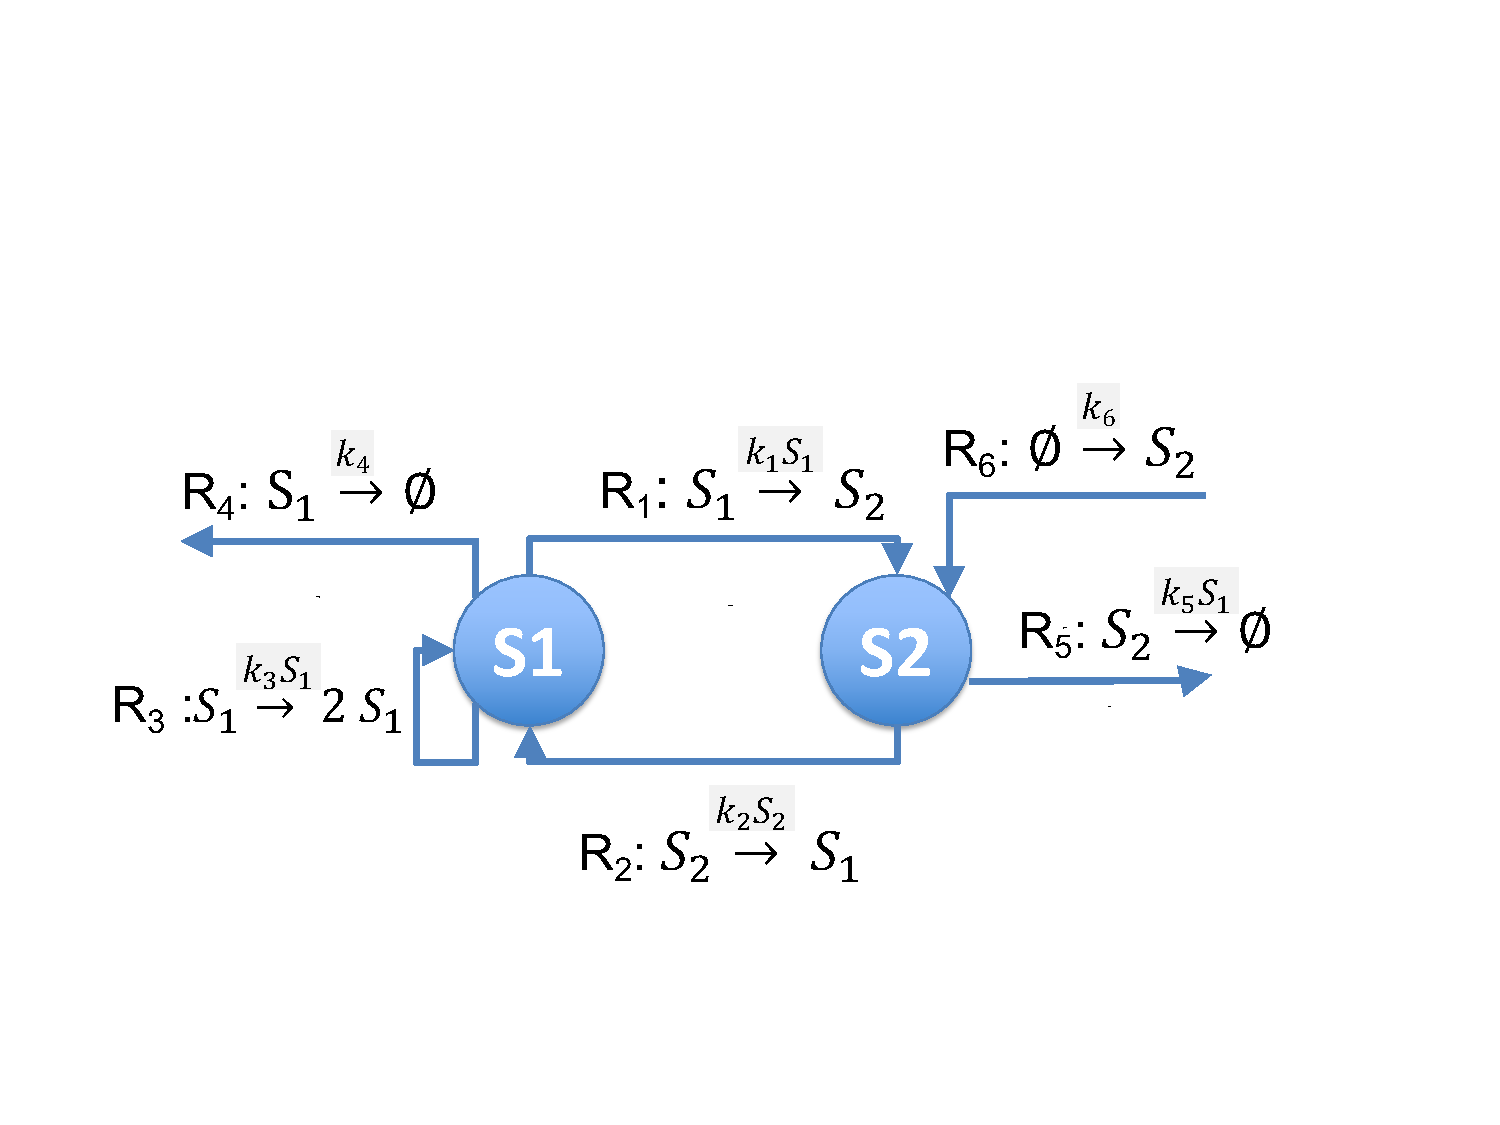
\includegraphics[scale=0.5]{figures/Fig1.pdf}
         \caption[]{Reaction network that creates oscillations in the chemical species $S_1, S_2$. The reaction network is designed so that its time domain solution is a system of linear differential equations. The text describes constraints on the kinetic constants ($k_i$) and initial conditions of the chemical species to create an oscillator such that species concentrations are non-negative, a requirement for biological feasibility.} 
         \label{fig:reaction-network}
\end{figure}
%%%%%%%%%%%%%%%%%%%%%%%%%%%%%%%%

%%%%%%%%%%%%%%% reaction-network
\begin{figure}
{\tt
{\bf function designOscillator($\theta^{\star}, \alpha^{\star}, \phi^{\star}, \omega^{\star}$)}
\begin{enumerate}

\item
Construct the reference signal:
$x^{\star}(t) = \alpha^{\star} sin(t \theta^{\star} + \phi^{\star}) + \omega^{\star}$.

\item
$\mathcal{P} ({\theta}) = \mathcal{P} \text{ with } k_d = \frac{(\theta^{\star})^2}{k_2}.$

\item Given $\mathcal{P} (\theta)$, we calculate $x_n(t; \mathcal{P}(\theta))$, the concentrations of $S_n$ using the formulas in \tab{tab:oc}. From this, we calculate the loss functions using relaxation (item (b) below):
\begin{enumerate}
\item
$L_n (\mathcal{P} ({\theta}))= \sum_t \delta(t) \left( x^{\star}(t) - x_n(t; \mathcal{P}(\theta)) \right)^2$
\item where $\delta(t) = 1$ if $x_n (t; \mathcal{P}(\theta))  \geq 0$; otherwise, $\delta$ is a large number.
\end{enumerate}

\item Find
$\hat{\mathcal{P}}_n (\theta) = argmin_{\mathcal{P}(\theta)} L_n (\mathcal{P} (\theta))$

\item Select the independent parameters.
\begin{enumerate}
\item If $L_1 (\hat{\mathcal{P}}_1 (\theta)) < L_2 (\hat{\mathcal{P}}_2 (\theta))$, return $\hat{\mathcal{P}}_1 (\theta)$
\item Else return $\hat{\mathcal{P}}_2 (\theta)$
\end{enumerate}

\end{enumerate}
}
\caption{Algorithm for finding values of parameters of the reaction network that achieve desired oscillations. The function {\tt designOscillator} takes
as inputs the desired oscillator characteristics and returns the independent parameters $\mathcal{P} (\theta)$ for
the reaction network: $k_2, k_4, k_6, x_1(0), x_2(0)$.
In essence, {\tt designOscillator}
inverts $x_n (t)$ by finding the $\mathcal{P}$ that minimizes
the squared error difference between the desired oscillations and $x_n (t)$ for either
$n=1$ or $n=2$.
In step 2, ``relaxation" (via $\delta (t)$) 
is used to address the hard constraints that $x_n (t) \geq 0$.}
\label{fig:design-oscillator}
\end{figure}
%%%%%%%%%%%%%%%%%%%%%%%%%%%%%%%%

%%%%%%%%%%%%%%% model-evaluation
\begin{figure}
        \centering
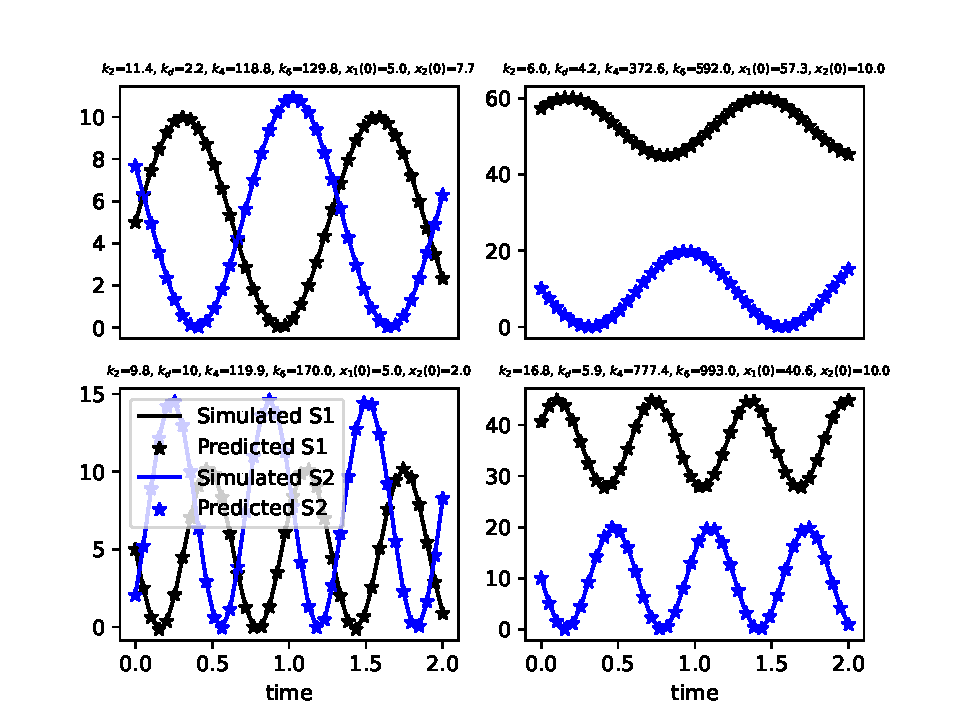
\includegraphics[scale=0.75]{figures/evaluate_model.pdf}
         \caption{Evaluations of model accuracy.
         Plots of simulation results (solid lines)
         and model predictions (markers) using the formulas in \tab{tab:oc} for four sets of parameter values of
         the reaction network in \fig{fig:reaction-network}.
         In all cases, predictions coincide with the simulation results.
         The four cases have different values for the
         the independent parameters; dependent parameters are calculated as described in the text.
         The initial value of $S_n$ is $x_n (0)$.}
         \label{fig:model-evaluation}
\end{figure}
%%%%%%%%%%%%%%%%%%%%%%%%%%%%%%%%


%%%%%%%%%%%%%%% amplitude-design-error-x1
\begin{figure}
        \centering
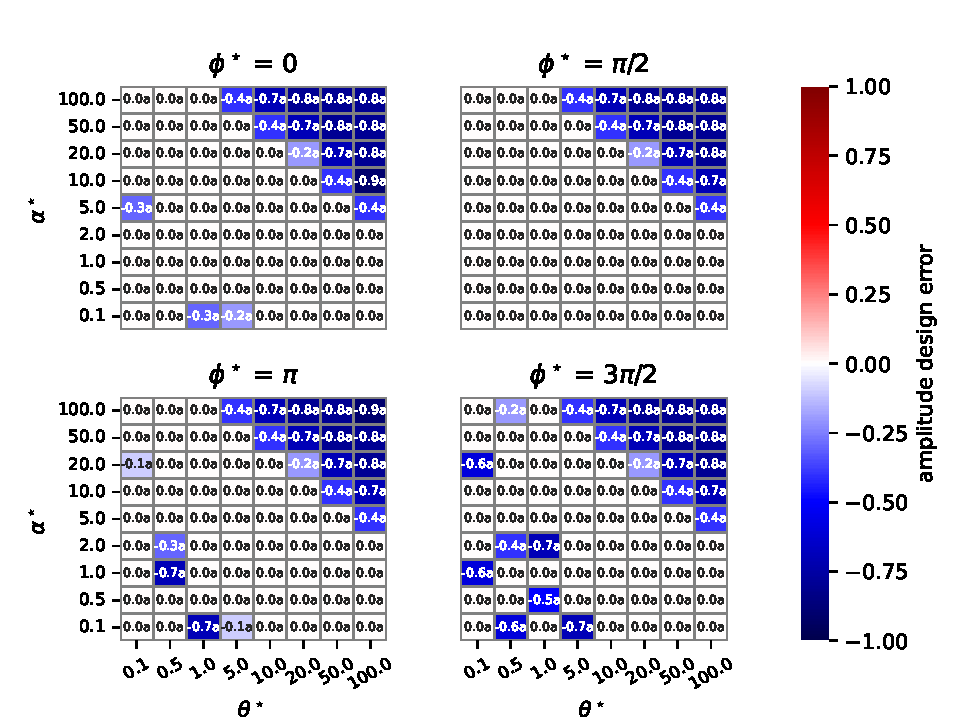
\includegraphics[scale=0.75]{figures/evaluation_plot_alphadev_x1.pdf}
         \caption[]{Amplitude design errors when {\tt designOscillator} in \fig{fig:design-oscillator} is modified so that $S_1$ is always the oscillating species. The heatmaps display amplitude design errors for four phases ($\phi^{\star}$). In each heatmap, the horizontal axis is desired frequency ($\theta^{\star}$), and the vertical axis is desired amplitude ($\alpha^{\star}$). Cell colors indicate the magnitude of the amplitude design error, and cells are annotated with the actual value. The letter ``a" indicates that species $S_1$ is the oscillating species.} 
         \label{fig:amplitude-design-error-x1}
\end{figure}
%%%%%%%%%%%%%%%%%%%%%%%%%%%%%%%%


%%%%%%%%%%%%%%% amplitude-design-error-both
\begin{figure}
        \centering
         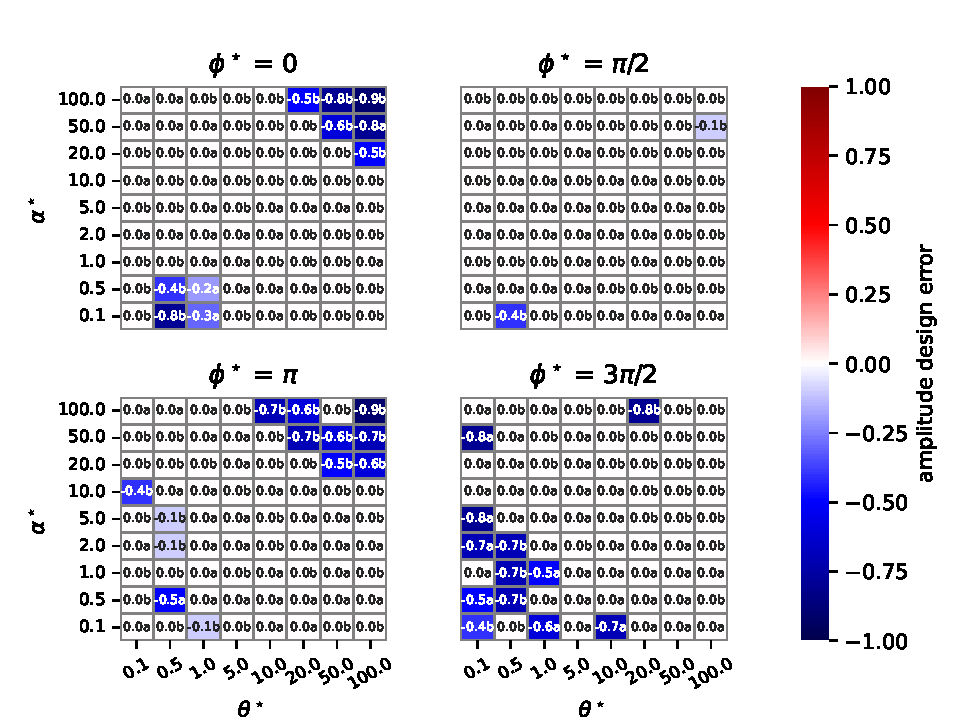
\includegraphics[scale=0.75]{figures/evaluation_plot_alphadev_both.pdf}
         \caption[]{Amplitude design errors are reduced when {\tt designOscillator} is used as-is so that either $S_1$ or $S_2$ can be the oscillating species. The heatmaps are structured as in \fig{fig:amplitude-design-error-x1}. The letter ``a" indicates that species $S_1$ is the oscillating species, and ``b" indicates that $S_2$ is the oscillating species.} 
         \label{fig:amplitude-design-error-both}
\end{figure}
%%%%%%%%%%%%%%%%%%%%%%%%%%%%%%%%


%%%%%%%%%%%%%%% phase-design-error-both
\begin{figure}
        \centering
         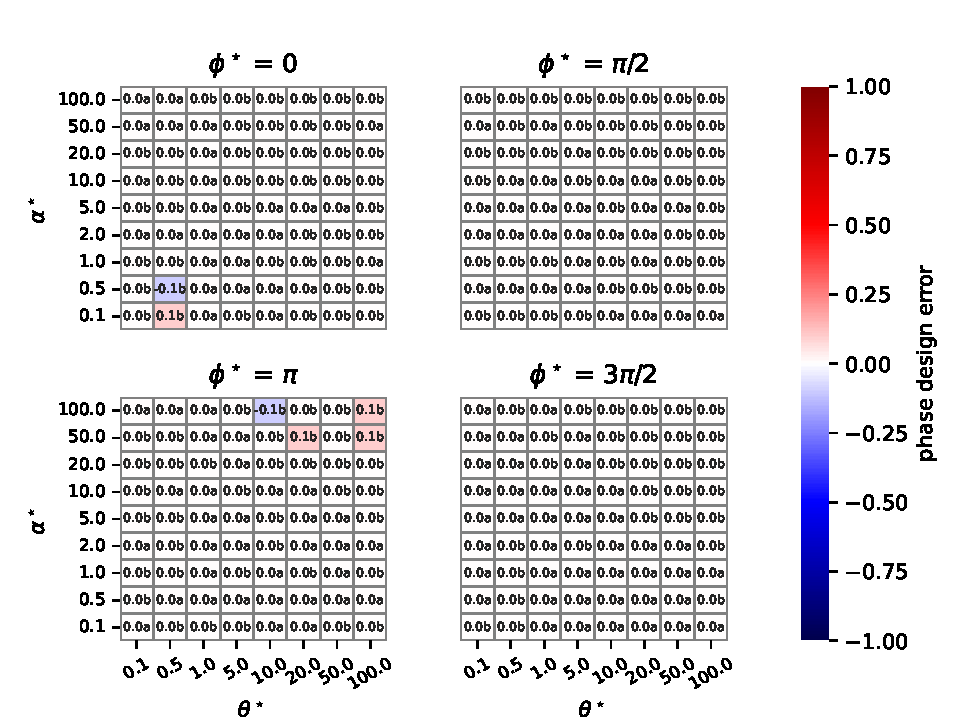
\includegraphics[scale=0.75]{figures/evaluation_plot_phidev_both.pdf}
         \caption[]{Phase design error. These heatmaps are organized in the same way as \fig{fig:amplitude-design-error-x1}, but cell values are phase design errors, the fraction of a cycle that the phase of the designed network differs from the phase of the desired oscillations. {\tt designOscillator} almost always produces a phase design error of 0.} 
         \label{fig:phase-design-error-both}
\end{figure}
%%%%%%%%%%%%%%%%%%%%%%%%%%%%%%%%


%%%%%%%%%%%%%%% histogram-of-parameter-values
\begin{figure}
        \centering
         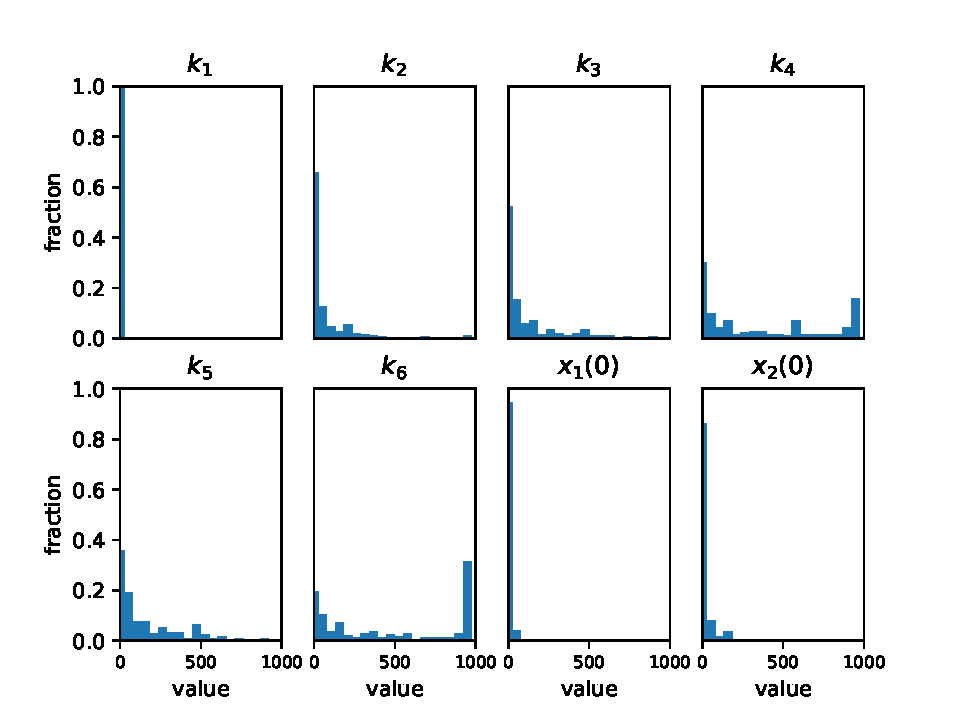
\includegraphics[scale=0.75]{figures/histogram_plot_both.pdf}
         \caption[]{Histograms of values of parameter estimates in the numerical studies. The algorithm limits parameter values to the range $[0, 1000]$. Only the parameters associated with the boundary reactions $R_4$ ($k_4$) and $R_6$ ($k_6$) have values close to the upper bound of this range. These larger values are needed to construct oscillators that produce large amplitudes and high frequencies.} 
         \label{fig:histogram-of-parameter-values}
\end{figure}
%%%%%%%%%%%%%%%%%%%%%%%%%%%%%%%%

%\begin{figure}[h!]
%  \caption{Sample figure title}
%\end{figure}

%\begin{figure}[h!]
%  \caption{Sample figure title}
%\end{figure}

%%%%%%%%%%%%%%%%%%%%%%%%%%%%%%%%%%%
%%                               %%
%% Tables                        %%
%%                               %%
%%%%%%%%%%%%%%%%%%%%%%%%%%%%%%%%%%%

%%%%%%%%%%%%%%%%%%%% tab:oc
\begin{table}[]
    \centering
    \begin{tabular}{||c|c||}
    \hline 
    & \\
    OCs & Formula \\
    & \\
    \hline
     & \\
          $\alpha_1$ & 
          $\frac{\sqrt{\theta^{2} \left(k_{2}^{2} x_1 (0) 
            + k_{2}^{2} x_2 (0) 
            - k_{2} k_{4} + k_{2} k_{d} x_1 (0) 
            - k_{4} k_{d} 
            + \theta^{2} x_2 (0)\right)^{2} 
          + \left(k_{2}^{2} k_{4} - k_{2}^{2} k_{6} 
            + k_{2} k_{4} k_{d} 
            + k_{2} \theta^{2} x_1 (0) 
            - k_{6} \theta^{2} 
            + k_{d} \theta^{2} x_1 (0)\right)^{2}}}
            {\theta^{2} \left(k_{2} + k_{d}\right)}$  \\ & \\
         $\alpha_2$ & 
           $\frac{\sqrt{\theta^{2} \left(k_{2} x_1 (0) 
           + k_{2} x_2 (0) 
           - k_{6} 
           + k_{d} x_1 (0)\right)^{2} 
           + \left(k_{2} k_{4} 
           - k_{2} k_{6} 
           + k_{4} k_{d} 
           - \theta^{2} x_2 (0)\right)^{2}}}
         {\theta^{2}}$  \\
          & \\
         $\theta$ & $\sqrt{k_2 k_d}$ \\
          & \\
          $\phi_1$ & $\operatorname{tan^{-1}}{\left(\frac{k_{2}^{2} k_{4} - k_{2}^{2} k_{6} + k_{2} k_{4} k_{d} + k_{2} \theta^{2} x_1 (0) - k_{6} \theta^{2} + k_{d} \theta^{2} x_1 (0)}{\theta \left(k_{2}^{2} x_1 (0) + k_{2}^{2} x_2 (0) - k_{2} k_{4} + k_{2} k_{d} x_1 (0) - k_{4} k_{d} + \theta^{2} x_2 (0)\right)} \right)} + \pi_1$ \\
         
         & \\
         $\phi_2$ & $\operatorname{tan^{-1}}{\left(\frac{k_{2} k_{4} - k_{2} k_{6} + k_{4} k_{d} - \theta^{2} x_2 (0)}{\theta \left(k_{2} x_1 (0) + k_{2} x_2 (0) - k_{6} + k_{d} x_1 (0)\right)} \right)} + \pi_2 $ \\
         & \\
         $\omega_1$ & $\frac{- k_{2}^{2} k_{4} + k_{2}^{2} k_{6} - k_{2} k_{4} k_{d} + k_{6} \theta^{2}}{\theta^2 (k_{2} + k_{d})}$ \\
         & \\
         $\omega_2$ & $\frac{k_{2} k_{4} - k_{2} k_{6} + k_{4} k_{d}}{\theta^{2}}$ \\
         & \\
         \hline
    \end{tabular}
    \vspace{0.05in}
    \caption{Formulas for oscillator characteristics (OCs) in terms of the kinetic constants $k_i$ of the reaction network in \fig{fig:reaction-network} and the initial concentrations of the chemical species, $x_n(0)$ for species $S_n$. The formulas are obtained by solving the system of equations for the reaction network. The oscillator characteristics (OCs) are: amplitude ($\alpha_n$), frequency ($\theta$), phase ($\phi_n$), and DC offset ($\omega_n$). The terms $\pi_1, \pi_2$ are defined in the text, and reflect technical details related to the inverting the tangent function.} 
    \label{tab:oc}
\end{table}
%%%%%%%%%%%%%%%%%%%%%%%%

%% Use of \listoftables is discouraged.
%%
%\section*{Tables}
%\begin{table}[h!]
%\caption{Sample table title. This is where the description of the table %should go}
%  \begin{tabular}{cccc}
%    \hline
%    & B1  &B2   & B3\\ \hline
%    A1 & 0.1 & 0.2 & 0.3\\
%    A2 & ... & ..  & .\\
%    A3 & ..  & .   & .\\ \hline
%  \end{tabular}
%\end{table}

%%%%%%%%%%%%%%%%%%%%%%%%%%%%%%%%%%%
%%                               %%
%% Additional Files              %%
%%                               %%
%%%%%%%%%%%%%%%%%%%%%%%%%%%%%%%%%%%

%\section*{Additional Files}
%  \subsection*{Additional file 1 --- Sample additional file title}
%    Additional file descriptions text (including details of how to
%    view the file, if it is in a non-standard format or the file extension). % This might
%    refer to a multi-page table or a figure.
%
%  \subsection*{Additional file 2 --- Sample additional file title}
%    Additional file descriptions text.

\end{backmatter}
\end{document}
